% Chapter Performance Evaluation

\chapter{Performance Evaluation} % Main chapter title
\label{performance} % For referencing the chapter elsewhere, use \ref{performance}
This chapter has been divided into two sections: First section \ref{perf:apna_ms} is related to micro-benchmarking of the APNA Management Service and second section \ref{perf:scionlab} pertains to experiments conducted on SCIONLab related to bandwidth and latency.

\section{APNA Management Service Microbenchmark} \label{perf:apna_ms}
\subsection{EphID Generation}
\paragraph{Goal}
The goal of this experiment was to benchmark different function involved in the process of EphID generation and try to get an idea which is the most the expensive function in term of computation time.
\paragraph{Experimental Setup}
APNA Management service is running on server located in the Z\"urich with the following specification.
\begin{itemize}
    \item \textbf{Processor:} Intel(R) Xeon(R) CPU E5540  @ 2.53GHz
    \item \textbf{Core:} 6
    \item \textbf{RAM:} 8 GB
\end{itemize}
Client is a Raspberry Pi Model 3B with Quad Core 1.2GHz Broadcom BCM2837 64-bit CPU and 1 GB RAM.
\paragraph{Results}
We can see that from Figure \ref{fig:perf_ephid} and Figure \ref{fig:perf_ephid_dist} certificate generation (84.4\%) is the most expensive process as compared host id generation (3.1\%) and encrypting host id (12.5\%). This was an expected behavior because certificate generation involves complex asymmetric cryptographic task of signing the certificate. While on other hand encrypting host id involves symmetric cryptography using AES-CBC encryption mode. And as a general rule of thumb asymmetric cryptography is always more expensive than symmetric cryptography.
\begin{figure}[th!!]
\centering
\noindent
\makebox[\textwidth]{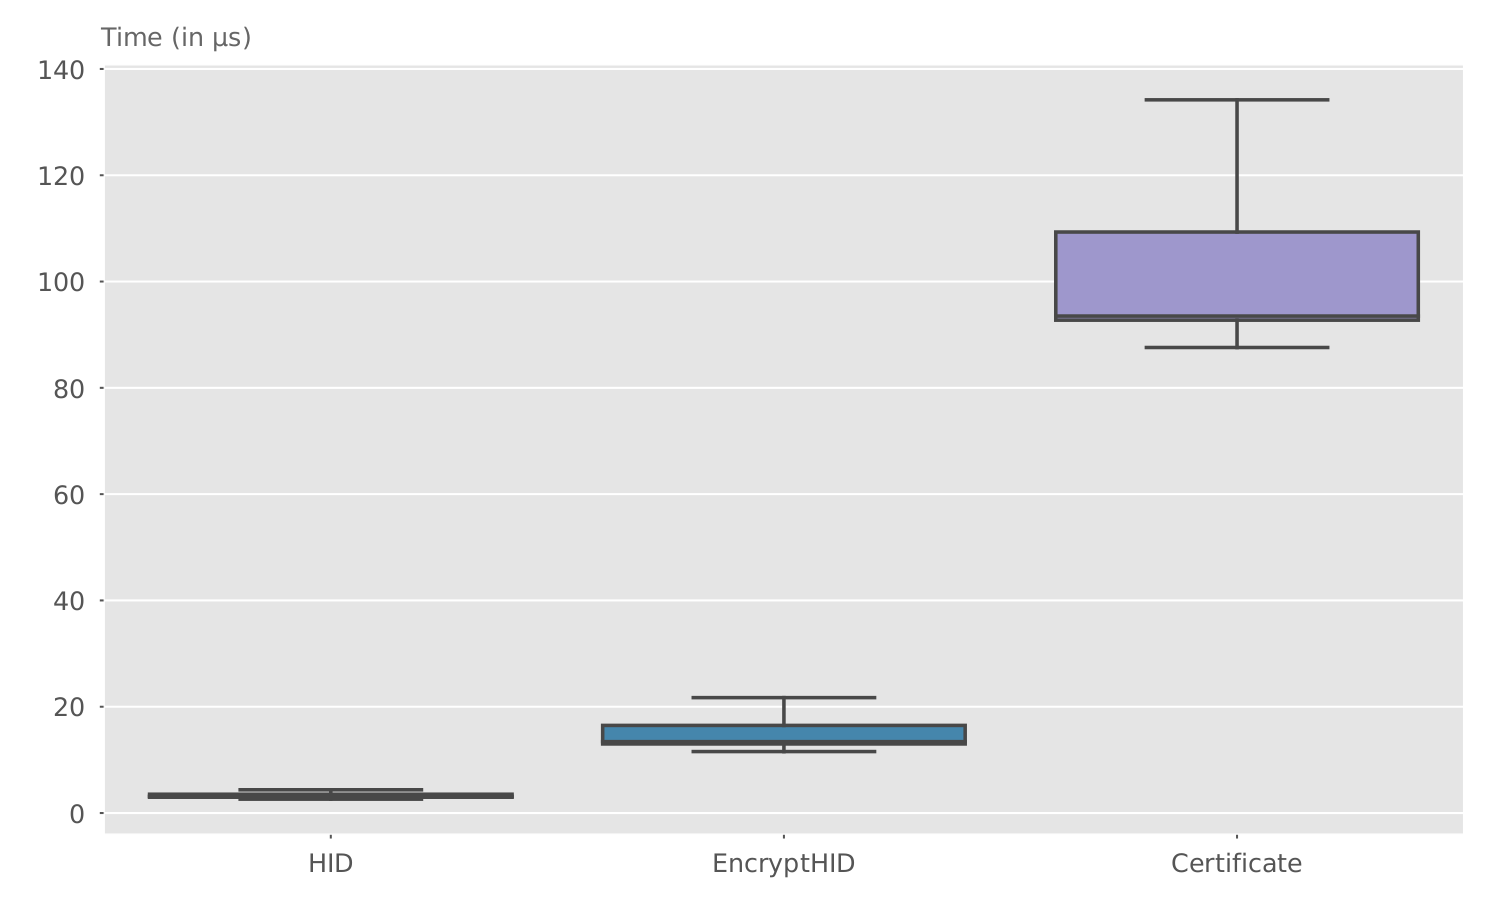
\includegraphics[scale=0.3]{Figures/ephid_gen_stat.png}}
\decoRule
\caption[EphID Generation Ops]{Time taken by different operation involved in EphID generation}
\label{fig:perf_ephid}
\end{figure}

\begin{figure}[th!!]
\centering
\noindent
\makebox[\textwidth]{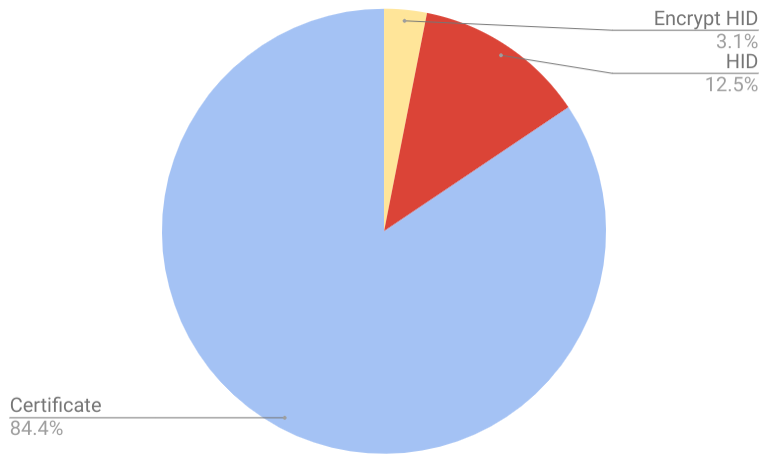
\includegraphics[scale=0.4]{Figures/distribution.png}}
\decoRule
\caption[EphID Generation Ops Distribution]{Percentage of time taken by different operation involved in EphID generation}
\label{fig:perf_ephid_dist}
\end{figure}

\section{DNS Microbenchmark}

\subsection{Goal}
The Goal of this experiment is to benchmark various operation related to DNS namely: a) DNS Domain Name Registration b) DNS Domain Name Resolution. Currently DNS is implemented using a simple Golang map data structure whose key is the domain name and value is the certificate issued for the Control EphID of the server.

\subsection{Experimental Setup}
There are two different experiments in order to achieve above goal. In the first experiment we are trying to benchmark the rate at which we can register domain names with the DNS Service. 10k domains names were registered with the DNS server while running this experiment. In the second experiment we are trying to benchmark the amount of time DNS server would take to respond to a query if its populated with 10k domain names. Each experiment was repeated 5 times for statistical significance.
\paragraph{Hardware Specification}
DNS service is running on server located in the Z\"urich with the following specification.
\begin{itemize}
    \item \textbf{Processor:} Intel(R) Core(TM) i7-7820X CPU @ 3.60GHz
    \item \textbf{Core:} 16
    \item \textbf{RAM:} 16 GB
\end{itemize}
Client is a Raspberry Pi Model 3B with Quad Core 1.2GHz Broadcom BCM2837 64-bit CPU and 1 GB RAM.
\begin{figure}[th!!]
\centering
\noindent
\makebox[\textwidth]{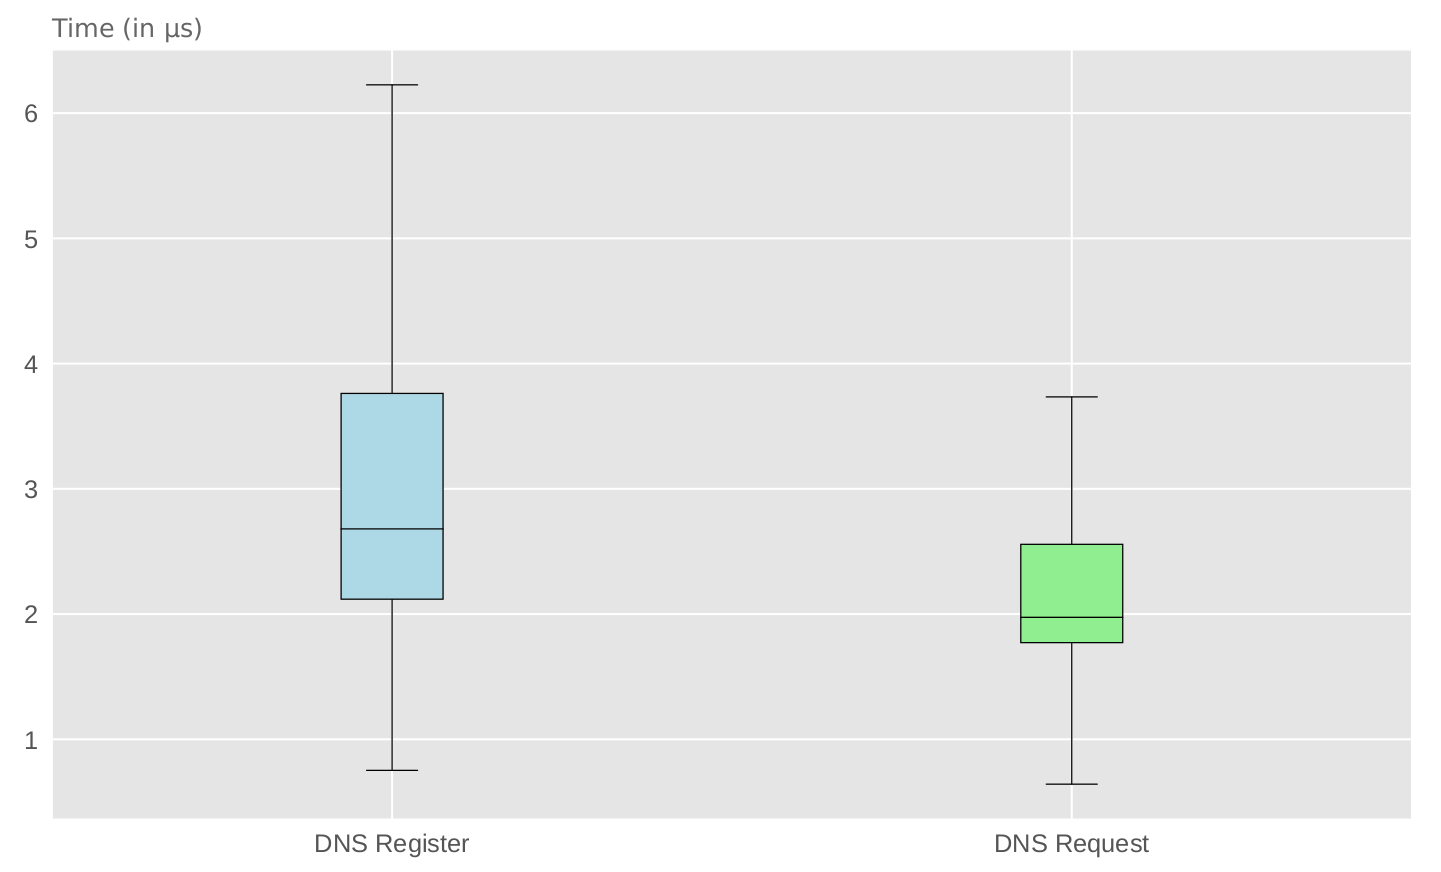
\includegraphics[scale=0.3]{Figures/dns_bench.png}}
\decoRule
\caption[DNS Operations]{Time taken by APNA MS for DNS Register and Request}
\label{fig:perf_dns}
\end{figure}

\subsection{Results}
As we can see in Figure \ref{fig:perf_dns} the amount of time it takes is in the order of few microseconds which is kind of an expected behavior as map inside Golang are implemented as hashmap and thus the complexity of insertion and lookup for hashmap is $\mathcal{O}(1)$ 

\section{Key Management Service Microbenchmark}

\subsection{Goal}
The goal of this experiment is to benchmark key management service of APNA Management Service. Key Management Service performs two major functions namely a) register host symmetric key b) reply to border router/APNA Service with the host symmetric key. Key Management Service is also implemented using simple Golang map data structure whose key is the host id and value is the symmetric key registered by the host for packet authentication.

\subsection{Experimental Setup}
There are two different experiments in order to achieve above goal. In the first experiment we are trying to benchmark the rate at which we can register host's symmetric key with the Key Management Service. 10k host's symmetric keys were registered with the Key Management server while running this experiment. In the second experiment we are trying to benchmark the amount of time Key Management server would take to respond to a query if its populated with 10k keys. Each experiment was repeated 5 times for statistical significance.
\paragraph{Hardware Specification}
Key Management service is running on server located in the Z\"urich with the following specification.
\begin{itemize}
    \item \textbf{Processor:} Intel(R) Core(TM) i7-7820X CPU @ 3.60GHz
    \item \textbf{Core:} 16
    \item \textbf{RAM:} 16 GB
\end{itemize}
Client is a Raspberry Pi Model 3B with Quad Core 1.2GHz Broadcom BCM2837 64-bit CPU and 1 GB RAM.

\begin{figure}[th!!]
\centering
\noindent
\makebox[\textwidth]{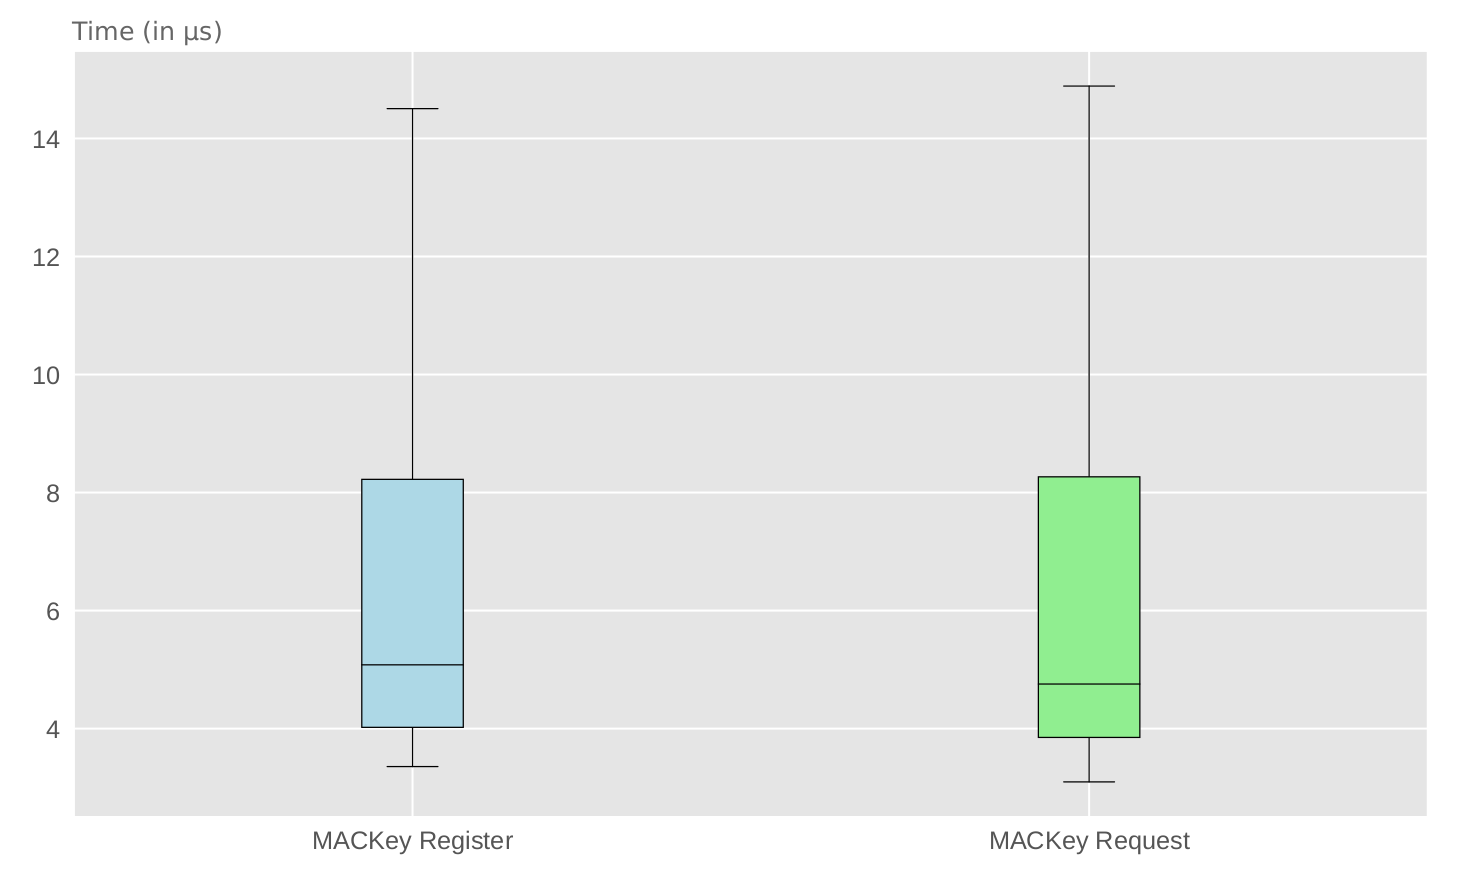
\includegraphics[scale=0.3]{Figures/mac_bench.png}}
\decoRule
\caption[MACKey Operations]{Time taken by APNA MS for MACKey Register and Request}
\label{fig:perf_mac}
\end{figure}

\subsection{Results}
As we can see in Figure \ref{fig:perf_mac} the amount of time it takes is in the order of few microseconds which is kind of an expected behavior as map inside Golang are implemented as hashmap and thus the complexity of insertion and lookup for hashmap is $\mathcal{O}(1)$ 

\section{Identity Management Service Microbenchmark}
\subsection{Goal}
The goal of this experiment is to benchmark identity management service of APNA Management Service. Key Management Service performs two major functions namely a) register host identity b) reply to border router/APNA Service with the host's IP addresss. Identity Management Service is also implemented using simple Golang map data structure whose key is the host id and value is the IP address associated with that host identity.

\subsection{Experimental Setup}
There are two different experiments in order to achieve above goal. In the first experiment we are trying to benchmark the rate at which we can register IP addresses with the Identity Service. 10k IP addresses were registered with the Identity Management Service while running this experiment. In the second experiment we are trying to benchmark the amount of time Identity Management Service would take to respond to a query if its populated with 10k Host IDs. Each experiment was repeated 5 times for statistical significance.

\paragraph{Hardware Specification}
Identity Management service is running on server located in the Z\"urich with the following specification.
\begin{itemize}
    \item \textbf{Processor:} Intel(R) Core(TM) i7-7820X CPU @ 3.60GHz
    \item \textbf{Core:} 16
    \item \textbf{RAM:} 16 GB
\end{itemize}
Client is a Raspberry Pi Model 3B with Quad Core 1.2GHz Broadcom BCM2837 64-bit CPU and 1 GB RAM.

\begin{figure}[th!!]
\centering
\noindent
\makebox[\textwidth]{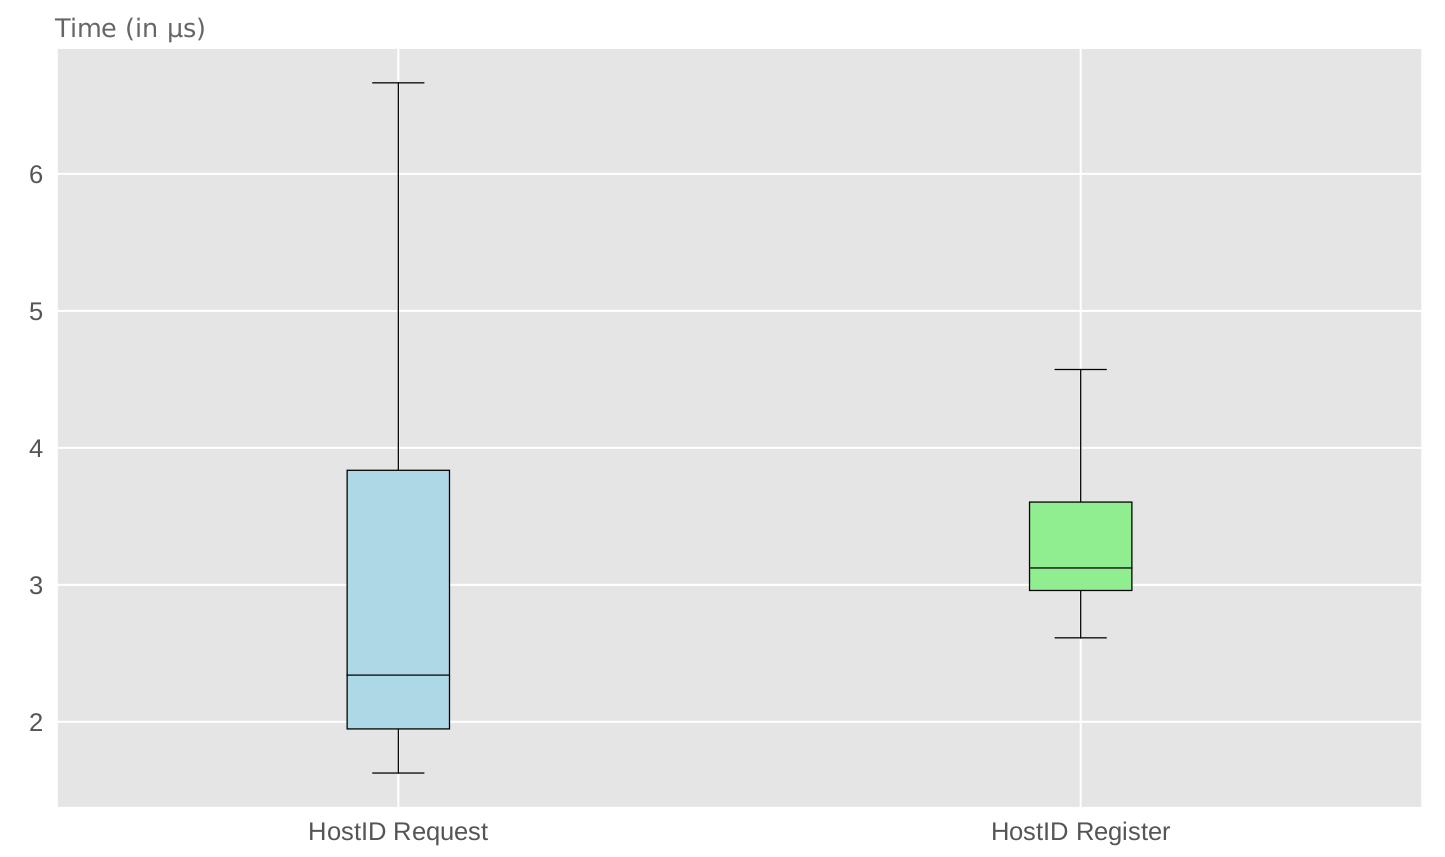
\includegraphics[scale=0.3]{Figures/hid_bench.png}}
\decoRule
\caption[HostID Operations]{Time taken by APNA MS for HostID Register and Request}
\label{fig:perf_hid}
\end{figure}

\subsection{Results}
As we can see in Figure \ref{fig:perf_hid} the amount of time it takes for both the operations is in the order of few microseconds which is kind of an expected behavior as map inside Golang are implemented as hashmap and thus the complexity of insertion and lookup for hashmap is $\mathcal{O}(1)$. Secondly the hashing algorithm used to generate Host ID is SipHash \cite{siphash} which itself is one of the fastest algorithm for hashing. The reason we see a slighter higher time for Host ID request because it involves two operations: a) Hashing of IP address and 2) Adding HID to the map.

\section{SCIONLab Benchmarks} \label{perf:scionlab}
\subsection{Objective}
In order to assess the overhead because of all the cryptographic operations performed inside APNA protocol. We tried to conduct bandwidth and latency experiments between APNA-SCION and vanilla-SCION (i.e., unmodified SCION). In order to assess the overhead we had three criteria. For these experiments we deployed ASes in two different ISD namely ISD-17 (Geographic Location: Switzerland) and ISD-20 (Geographic Location: South Korea). Geographical all the AS's VM are located in Switzerland.
\begin{itemize}
    \item ASes attached to different ISDs (i.e., AS: \texttt{17-ffaa:1:c7} and AS: \texttt{20-ffaa:1:cb})
    \item ASes attached to the same ISD (i.e., AS: \texttt{17-ffaa:1:c7} and AS: \texttt{17-ffaa:1:d5})
    \item ASes attached to the same ISD but geographical location of ISD and ASes are different (i.e., AS: \texttt{20-ffaa:1:cb} and AS: \texttt{20-ffaa:1:d4})
\end{itemize}

\subsection{Experimental Setup}
Two ASes have been deployed on PC-engine and the other two have been deployed using a SCION-VM provided by SCIONLab.

\paragraph{Hardware specification of PC-Engine}
\begin{itemize}
    \item \textbf{Processor:} AMD GX-412TC SOC @ 600 MHz
    \item \textbf{Core:} 4
    \item \textbf{RAM:} 4 GB
\end{itemize}

\paragraph{Hardware specification of VM}
\begin{itemize}
    \item \textbf{Processor:} Intel(R) Core(TM) i7-7820X CPU @ 3.60GHz
    \item \textbf{Core:} 2
    \item \textbf{RAM:} 2 GB
\end{itemize}

\subsection{Latency Benchmarks}
\paragraph{Experimental Setup}
There are two different cases:
\begin{itemize}
    \item \textbf{APNA-SCION }\\ Client sends a 4 bytes ("ping") message to the server by encrypting it. Once the server receives the message it decrypts and check the content of the message. If the message contains "ping" then server replies back with 4 bytes message ("pong") to the client. Client decrypts the message and check the contents of the message as well. The amount of time it took to perform the aforementioned procedure is measured as Round Trip Time (RTT) for the APNA.
    \item \textbf{VANILLA-SCION} \\ For vanilla SCION there is already an application called \texttt{pingpong} which can be used to measure RTT on SCION. 
\end{itemize}

\begin{figure}[th!!]
\centering
\noindent
\makebox[\textwidth]{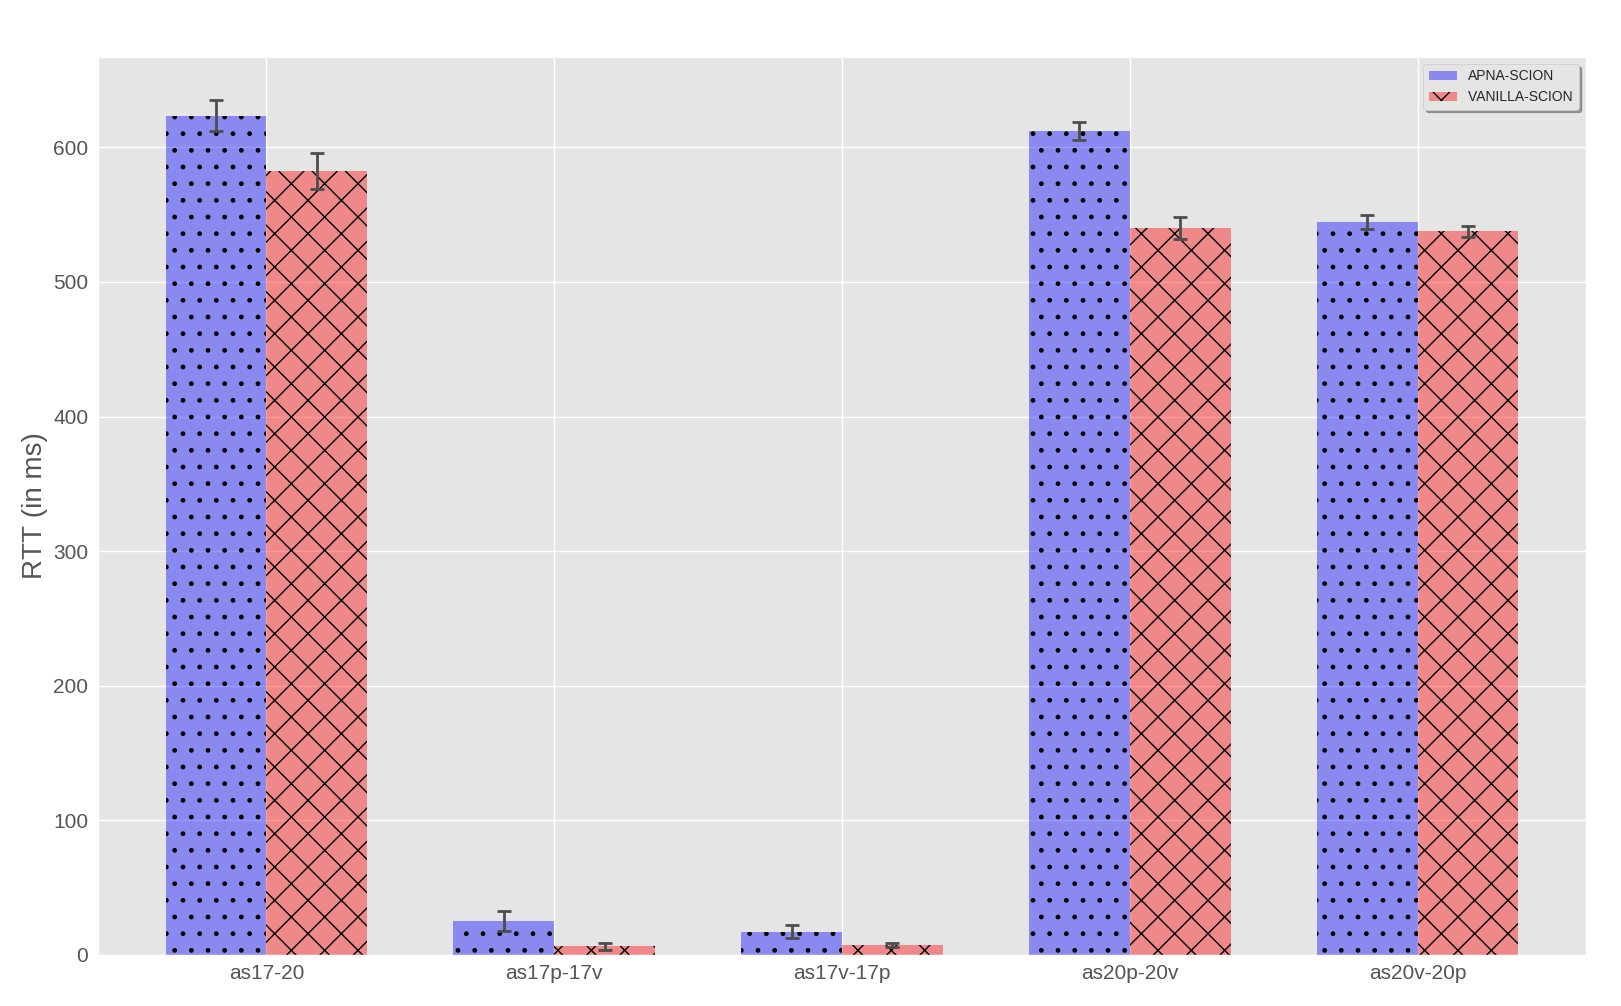
\includegraphics[scale=0.3]{Figures/lat_test.png}}
\decoRule
\caption[Latency Analysis]{Latency Analysis for Vanilla SCION and APNA SCION}
\label{fig:perf_latency}
\end{figure}

\paragraph{Results}
Figure \ref{fig:perf_latency} presents some interesting insights about how APNA affects RTT. In terms of absolute number there is a overhead of around 10-60 \% for using APNA that is mostly because of the cost of encrypting and decrypting the packet. In the figure you can observe the effect of geographic location as well since ASes in ISD 17 have significantly lower RTT as compared to ASes located in ISD 20. ASes in ISD20 are physically located in Switzerland but attached to South Korea which redirects the packet first to Korea and then it comes back to Switzerland because of the IP overlay.

\subsection{Bandwidth Benchmarks}
Bandwidth is not easy to define concept specially when we are using unreliable transport medium such as UDP. Since there is no congestion control or flow control to handle the packets sent in burst. It would not be fair to measure to burst bandwidth we notice a lot of packet drop on the receiving side. We are more interested in steady bandwidth which results in acceptable amount of packet loss ($\leq$ 0.02\%). So we need a mechanisms to send packets at a uniform rate such that it does not create congestion in the network and results in a fewer packet drop.

\paragraph{Experimental Setup}
For both cases \textbf{APNA-SCION} and \textbf{VANILLA-SCION} client tries to probe for a bandwidth at which server observes an acceptable amount of packet loss ($\leq$ 0.02\%). It start off with a high number such as 100Mbps and calculate the amount of packet it needs to send in 1 sec to achieve that bandwidth using the current MTU (1320) size. After that its kind of similar to a binary search it reduce the bandwidth to half or double it depending upon whether the packet loss was more or less than acceptable amount of packet loss.

\begin{figure}[th!!]
\centering
\noindent
\makebox[\textwidth]{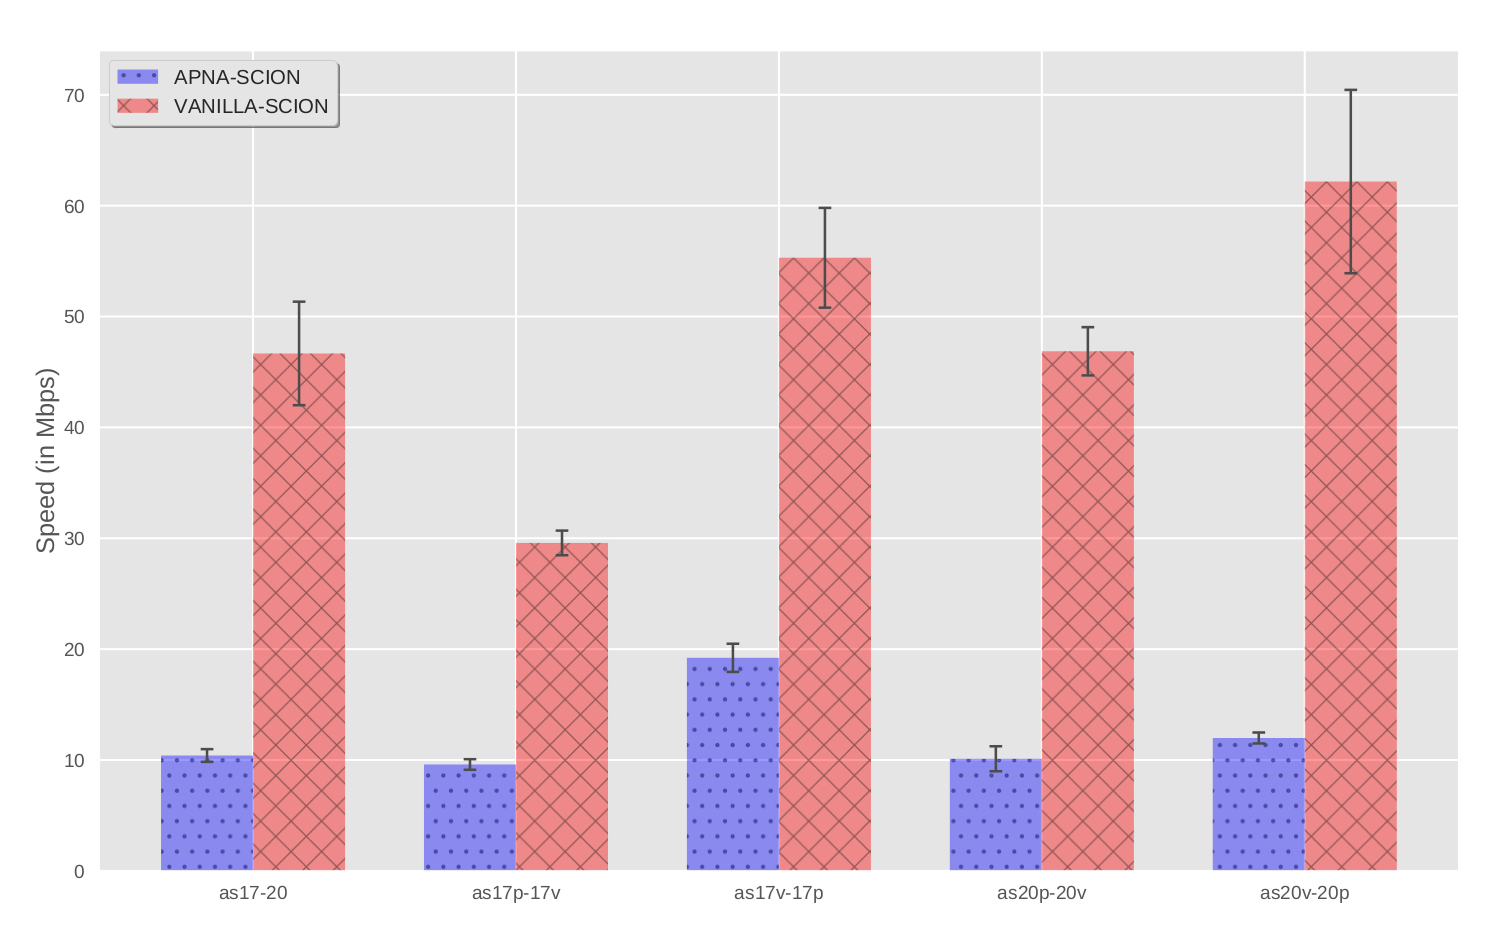
\includegraphics[scale=0.3]{Figures/bw_test.png}}
\decoRule
\caption[Bandwidth Analysis]{Bandwidth Analysis for Vanilla SCION and APNA SCION}
\label{fig:perf_bandwidth}
\end{figure}

\paragraph{Results}
Figure \ref{fig:perf_bandwidth} gives some interesting insights about the bandwidth. Bandwidth for VANILLA-SCION is 3-5x more than APNA-SCION which was an expected behavior since APNA performs a complete packet encryption which is requires a lot of CPU cycles since Golang version used for SCION development does not use hardware acceleration for faster encryption. Furthermore, there is an additional overhead of serializing and deserializing packets twice since the packet first goes to APNA service and then to the border router.